\documentclass[12pt]{article}

\usepackage{answers}
\usepackage{setspace}
\usepackage{graphicx}
\usepackage{enumitem}
\usepackage{multicol}
\usepackage{mathrsfs}
\usepackage[margin=1in]{geometry} 
\usepackage{amsmath,amsthm,amssymb}
\usepackage[english]{babel}

\newcommand{\N}{\mathbb{N}}
\newcommand{\Z}{\mathbb{Z}}
\newcommand{\C}{\mathbb{C}}
\newcommand{\R}{\mathbb{R}}

\DeclareMathOperator{\sech}{sech}
\DeclareMathOperator{\csch}{csch}

\newenvironment{theorem}[2][Theorem]{\begin{trivlist}
		\item[\hskip \labelsep {\bfseries #1}\hskip \labelsep {\bfseries #2.}]}{\end{trivlist}}
\newenvironment{definition}[2][Definition]{\begin{trivlist}
		\item[\hskip \labelsep {\bfseries #1}\hskip \labelsep {\bfseries #2.}]}{\end{trivlist}}
\newenvironment{proposition}[2][Proposition]{\begin{trivlist}
		\item[\hskip \labelsep {\bfseries #1}\hskip \labelsep {\bfseries #2.}]}{\end{trivlist}}
\newenvironment{lemma}[2][Lemma]{\begin{trivlist}
		\item[\hskip \labelsep {\bfseries #1}\hskip \labelsep {\bfseries #2.}]}{\end{trivlist}}
\newenvironment{exercise}[2][Exercise]{\begin{trivlist}
		\item[\hskip \labelsep {\bfseries #1}\hskip \labelsep {\bfseries #2.}]}{\end{trivlist}}
\newenvironment{solution}[2][Solution]{\begin{trivlist}
		\item[\hskip \labelsep {\bfseries #1}]}{\end{trivlist}}
\newenvironment{problem}[2][Problem]{\begin{trivlist}
		\item[\hskip \labelsep {\bfseries #1}\hskip \labelsep {\bfseries #2.}]}{\end{trivlist}}
\newenvironment{question}[2][Question]{\begin{trivlist}
		\item[\hskip \labelsep {\bfseries #1}\hskip \labelsep {\bfseries #2.}]}{\end{trivlist}}
\newenvironment{corollary}[2][Corollary]{\begin{trivlist}
		\item[\hskip \labelsep {\bfseries #1}\hskip \labelsep {\bfseries #2.}]}{\end{trivlist}}

\begin{document}
	\title{Robotics 1 - Summary}
	\author{Michael Gabler}
	\maketitle
	\tableofcontents
	\newpage
	
	\section{Basics}
	\subsection{Definitions}
	\textbf{Degrees of freedom}: Defines how many axes of the robot can be manipulated\\
	\textbf{Joints (Gelenke)}: The robot's joints can be \textbf{r}evolute (rotating) or \textbf{p}rismatic (expanding)\\
	\textbf{Joint variable}: The value that describes the state of the joint. This is the current length for prisamtic joints and the rotation angle for revolute joints.\\
	\textbf{Work envelope}: All points that can be reaced with the endeffector\\
	\textbf{Coordinate frames}: $[v]^M$ points out that the values of vector $v$ are in the coordinate frame $M$.
	
	\subsection{Mathematical Background}
	\paragraph{Sinus, Cosinus, Tangenz}
	Short formes: $S_{k} = \sin \theta_{k}$, $C_{k} = \cos \theta_{k}$\\
	$\arctan(\frac{y}{x}) \in ]-\frac{\pi}{2};\frac{\pi}{2}[$: to find all solutions use the $\arctan2$ instead:
	\begin{equation}
	\arctan2(y,x) = 
	\left\{ \begin{array}{ll}
	\arctan(\frac{y}{x}), & x > 0\\
	sgn(y)\frac{\pi}{2}, & x = 0\\
	\arctan(\frac{y}{x}) + sgn(y)\pi, & x < 0, y \neq 0\\
	\pi, & x < 0, y = 0
	\end{array} \right.
	\end{equation}
	
	\paragraph{Matrices and vectors}
	$I$: \textbf{Identitymatrix}, 0 for every element exept the diagonal from top left to bottom right\\
	\textbf{Inverse matrix} $M^{-1}$: $M^{-1} M = I$\\
	\textbf{Rank of the matrix}: is the number of row vectors that are not 0. Before that use the Gaussian elimination (change row vectors, add or subtract row vectors multiplied with a scalar to/from each other):
	\begin{equation}
	A = 
	\begin{bmatrix}
	1 & 2 & 3\\
	0 & 6 & 4\\
	0 & 3 & 2
	\end{bmatrix}
	\rightarrow
	\begin{bmatrix}
	1 & 2 & 3\\
	0 & 6 & 4\\
	0 & 0 & 0
	\end{bmatrix}
	\Rightarrow
	rank(A) = 2
	\end{equation}
	
	
	\subsection{Transformations}
	Describe how a coordinate frame is located in respect to a base reference frame.
	\paragraph{Fundamental rotation matrices} $R_{n}(\phi)$ describes the rotation around the n axes with the angle $\phi$.\\
	\begin{equation}
	R_{1}(\phi) = 
	\begin{bmatrix}
	1 & 0 & 0\\
	0 & \cos \phi & -\sin \phi\\
	0 & \sin \phi & \cos \phi
	\end{bmatrix}
	\end{equation}
	\begin{equation}
	R_{2}(\phi) = 
	\begin{bmatrix}
	\cos \phi & 0 & \sin \phi\\
	0 & 1 & 0\\
	-\sin \phi & 0 & \cos \phi
	\end{bmatrix}
	\end{equation}
	\begin{equation}
	R_{3}(\phi) = 
	\begin{bmatrix}
	\cos \phi & -\sin \phi & 0\\
	\sin \phi & \cos \phi & 0\\
	0 & 0 & 1
	\end{bmatrix}
	\end{equation}
	
	\paragraph{Yaw-Pitch-Roll transformation} Rotate around $f^1$ with $\theta_{1}$, $f^2$ with $\theta_{2}$ and $f^3$ with $\theta_{3}$
	\begin{equation}
	YPR(\theta) = 
	\begin{bmatrix}
	C_{2} C_{3} & S_{1} S_{2} C_{3} - C_{1} S_{3} & C_{1} S_{2} C_{3} + S_{1} S_{3}\\
	C_{2} S_{3}  & S_{1} S_{2} S_{3} + C_{1} C_{3} & C_{1} S_{2} S_{3} - S_{1} C_{3}\\
	-S_{2} & S_{1} C_{2} & C_{1} C_{2}
	\end{bmatrix}
	\end{equation}
	
	\paragraph{Euler Angles transformation} Rotate around $m^3$ with $\theta_{1}$, $m^2$ with $\theta_{2}$ and $m^3$ with $\theta_{3}$ again
	\begin{equation}
	R_{3}(\theta_{1}) R_{2}(\theta_{2}) R_{3}(\theta_{3}) = 
	\begin{bmatrix}
	C_{1} C_{2} C_{3} - S_{1} S_{3} & -C_{1} C_{2} S_{3} - S_{1} C_{3} & C_{1} S_{2}\\
	S_{1} C_{2} C_{3} + C_{1} S_{3}  & -S_{1} C_{2} S_{3} + C_{1} C_{3} & S_{1} S_{2}\\
	-S_{2} C_{3} & S_{2} S_{3} & C_{2}
	\end{bmatrix}
	\end{equation}
	
	\paragraph{Homogenous transformation} Describe coordinates as homogenous coordinates to describe rotations and translations\\
	vector $q$ as homogenous coordinates is $[q_{1} q_{2} q_{3} 1]^T$\\
	Homogenous transformation matrix
	\begin{equation}
	T = 
	\begin{bmatrix}
	R & p\\
	\eta^T & \sigma
	\end{bmatrix}
	\end{equation}
	with\\
	$R \in \R^{3 \times 3}$ is a rotation matrix\\
	$p \in \R^{3 \times 1}$ is a translation vector\\
	$\sigma \in \R$ is a scaling factor (usually 1)\\
	$\eta^T \in \R^{1 \times 3}$ is a perspective vector, here zero vector	\begin{equation}
	Rot(\phi, k) = 
	\begin{bmatrix}
	& & & 0\\
	& R_{k}(\phi) & & 0\\
	& & & 0\\
	0 & 0 & 0 & 1
	\end{bmatrix}, 
	Tran(p) = 
	\begin{bmatrix}
	1 & 0 & 0 & p_{1}\\
	0 & 1 & 0 & p_{2}\\
	0 & 0 & 1 & p_{3}\\
	0 & 0 & 0 & 1
	\end{bmatrix}
	\end{equation}
	
	Calculate arbitrary transformations by using the following rules:
	\begin{enumerate}
		\item Start with $T = I$, $F$ (fixed frame) and $M$ (mobile frame) are equivalent
		\item Represent rotations and translations as separate fundamental homogenous transformation matrices
		\item If $M$ is rotated about or translated along a unit vector of $F$, \textbf{premultiply} homogenous transformation matrix to $T$
		\item If $M$ is rotated about or translated along a unit vector of $M$, \textbf{postmultiply} homogenous transformation matrix to $T$
	\end{enumerate}
	
	% TODO: how to transform coodinates from one frame to another?
	
	\paragraph{Inverse homogenous transformation} If the transformation matrix $T$ maps coordinates from coordinate frame $A$ to $B$, the inverse $T^{-1}$ maps coodinates from $B$ to $A$.
	\begin{equation}
	T^{-1} = 
	\begin{bmatrix}
	& R^T & & -R^T p\\
	0 & 0 & 0 & 1
	\end{bmatrix}
	\end{equation}
	with $\eta = 0$ and $\sigma = 1$
	
	\paragraph{Screw transformation} rotation of $\phi$ and translation of $\lambda$ around/about the same axis $k$ (unit vector of $F$) like the movement with a screw driver
	\begin{equation}
	Screw(\lambda,\phi,k) = Rot(\phi , k) Tran(\lambda i^k)
	\end{equation}
	with $i^k$ as $k$-th unit vector
	
	\section{Manipulators}
	\subsection{Direct kinematics}
	Direct kinematics is the determination of the tool tip's coordinates and orientation in the base coordinate frame when the values for the joint variables are given.
	\subsubsection{Right-Hand Rules}
	The assignment of the axis of a coodinate frame follows the right-hand rule (see figure \ref{fig:right-hand-frame}).\\
	\begin{figure}[h]
		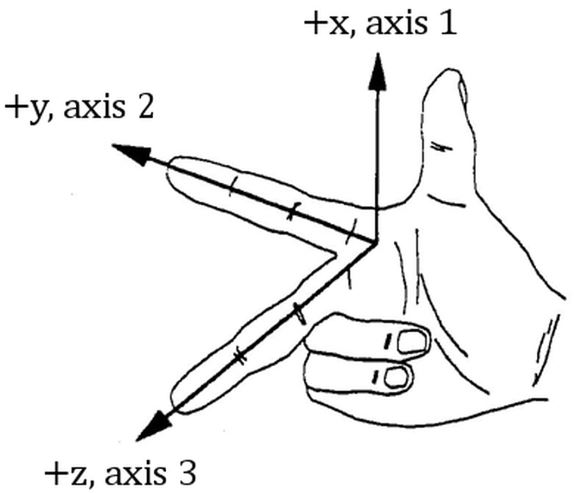
\includegraphics[width=0.5\textwidth]{figures/right-hand-frame.JPG}
		\caption{Right-handed coordinate frame}
		\label{fig:right-hand-frame}
	\end{figure}
	To determine the positive direction of a rotation angle use the right-hand rule by pointing the thumb in the positive direction of the rotation axis. The remaining fingers indicate the positive direction of rotation. (see figure \ref{fig:right-hand-rule})
	\begin{figure}[h]
		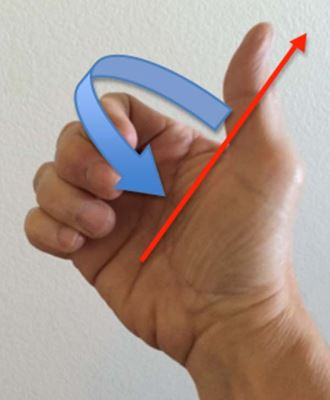
\includegraphics[width=0.5\textwidth]{figures/right-hand-rule.JPG}
		\caption{Right-hand rule}
		\label{fig:right-hand-rule}
	\end{figure}
	
	\subsubsection{Kinematic parameters}
	Specify the kinematic configuration of a robot. There are $4n$ parameters for a $n$-axis robot, 4 for each link/joint, one of them is variable and is called \textbf{joint variable}.
	
	\begin{tabular}{|l|c|c|c|}
		\hline
		\textbf{Arm parameter} & \textbf{Symbol} & \textbf{Revolute joint} & \textbf{Prismatic joint} \\ \hline
		Joint angle            &    $\theta$     &        variable         &          fixed           \\ \hline
		Joint distance         &       $d$       &          fixed          &         variable         \\ \hline
		Link length            &       $a$       &          fixed          &          fixed           \\ \hline
		Link twist angle       &    $\alpha$     &          fixed          &          fixed           \\ \hline
	\end{tabular} 
	
	\subsubsection{Denavit-Hartenberg Algorithm}
	The Denavit-Hartenberg Algorithm is used to assign coordinate frames to each link of the robot and to determine the kinematic parameters of the robot.\\
	Numbering of links: $0$ (fixed base) to $n$ at the tool $\Rightarrow$ $n+1$ links for $n$-axis robot\\
	Numbering of joints: joint $k$ interconnects link $k-1$ with link $k$ with $1 \leq k \leq n$
	\paragraph{Part 1: Assignment of coordinate frames}
	\begin{enumerate}
		\item Number the joints from $1$ to $n$
		\item Assign a right-handed orthonormal coordinate frame $L_0$ to robot base, making sure that $z^0$ aligns with the axis of joint $1$. Set $k = 1$.
		\item Align $z^k$ with the axis of joint $k + 1$.
		\item Locate the orign of $L_k$ at the intersection of the $z^k$ and $z^{k-1}$ axes.\\
		If they are not parallel and do not intersect, use the intersection of $z^k$ with a common normal between $z^k$ and $z^{k-1}$.\\
		If they are parallel, use the intersection of $z^k$ with either a normal between $z^k$ and $z^{k+1}$ or the normal between $z^k$ and $z^{k-1}$ intersecting the origin of $L_{k-1}$.
		\item Select $x^k$ to be orthogonal to both $z^k$ and $z^{k-1}$, making sure that $x^k$ intersects $z^{k-1}$. $x^k$ should point away from $z^{k-1}$.
		\item Select $y^k$ to form a right-handed orthonormal coordinate frame $L_k$.
		\item Set $k \leftarrow k + 1$. If $k < n$, go to step 3, else continue.
		\item Set the origin of $L_n$ at the tool tip. Align $z^n$ with the approach vector, $y^n$ with the sliding vector and $x^n$ with the normal vector of the tool.\\
		Set $k = 1$ and continue with part 2.
	\end{enumerate}
	\paragraph{Part 2: Determination of kinematic parameters}
	\begin{enumerate}
		\item Locate point $b_k$ at the intersection of the $x^k$ and $z^{k-1}$ axes.\\
		Only in case $k = n$: If they do not intersect, use the intersection of $x^k$ with a common normal between $x^k$ and $z^{k-1}$
		\item Compute $\theta_{k}$ as the angle of rotation from $x^{k-1}$ to $x^k$ measured about $z^{k-1}$.
		\item Compute $d_k$ as the distance from the origin of frame $L_{k-1}$ to point $b_k$ measured along $z^{k-1}$.
		\item Compute $a_k$ as the distance from point $b_k$ to the origin of frame $L_k$ measured along $x^k$.
		\item Compute $\alpha_k$ as the angle of rotation from $z^{k-1}$ to $z^k$ measured about $x^k$.
		\item Set $k \leftarrow k + 1$. If $k \leq n$, go to step 1, else stop.
	\end{enumerate}
	
	\subsubsection{Arm equation}
	The arm equation defines a transformation matrix $T^{tool}_{base}(q)$ that transforms coordinates of the tool coordinate frame $L_n$ to the base coordinate frame $L_0$ and depends on the vector of joint variables $q$ (see equation \ref{eq:transform-tool-base}). It is composed out of several transformations between the link coodinate frames (see equation \ref{eq:transform-lcf}).
	\begin{equation}
	T^{k}_{k-1} = 
	\begin{bmatrix}
	C \theta_k & -C \alpha_k S \theta_k & S \alpha_k S \theta_k & a_k C \theta_k\\
	S \theta_k & C \alpha_k C \theta_k & -S \alpha_k C \theta_k & a_k S \theta_k\\
	0 & S \alpha_k & C \alpha_k & d_k\\
	0 & 0 & 0 & 1
	\end{bmatrix}
	\label{eq:transform-lcf}
	\end{equation}
	\begin{equation}
	(T^{k}_{k-1})^{-1} = T^{k-1}_{k} = 
	\begin{bmatrix}
	C \theta_k & S \theta_k & 0 & -a_k\\
	-C \alpha_k S \theta_k & C \alpha_k C \theta_k & S \alpha_k & -d_k S \alpha_k\\
	S \alpha_k S \theta_k & -S \alpha_k C \theta_k & C \alpha_k & -d_k C \alpha_k\\
	0 & 0 & 0 & 1
	\end{bmatrix}
	\end{equation}
	\begin{equation}
	T^{tool}_{base}(q) = T^1_0(q_1) T^2_1(q_2) ... T^n_{n-1}(q_n) = 
	\begin{bmatrix}
	& R(q) & & p(q)\\
	0 & 0 & 0 & 1
	\end{bmatrix}
	\label{eq:transform-tool-base}
	\end{equation}
	$R(q) \in \R^{3 \times 3}$ the orientation of the tool as rotation matrix.\\
	The three columns of $R(q)$ are the three unit vectors of the tool frame in relation to the base frame.\\
	\\
	$p(q) \in \R^3$ the translation vector and therefore the position of the tool tip in relation to the base frame.
	
	\subsection{Inverse kinematics}
	Inverse kinematics describes the task to determine the robot's joint variables when the tool tip's coordinates and orientation (called the tool configuration) is given. There are often multiple solutions because the position can be reached by different alignment of the joints.
	
	\subsubsection{Tool-configuration space}
	To describe the tool tip's coordinates and orientation one can use a $\R^6$-vector which is called the tool-configuration vector $w$.\\
	\begin{equation}
	w = 
	\begin{bmatrix}
	w_1 \\ w_2 \\ w_3 \\ w_4 \\ w_5 \\ w_6
	\end{bmatrix} = 
	\begin{bmatrix}
	p \\ e^{\frac{q_n}{\pi}}r^3
	\end{bmatrix}
	\end{equation}
	with $p \in \R^3$ the translation vector of the arm equation's vector $T^{tool}_{base}$\\
	$q \in \R^n$ the vector of joint variables for a robot with $n$-joints\\
	$r^3 \in \R^3$ the third column vector of the rotation matrix $R$ from $T^{tool}_{base}$
	
	\subsubsection{Solving the inverse kinematic}
	Construct a vector $w$ by calculating the matrix $T^{tool}_{base}$ and taking the equations from there. $w_1, ..., w_6$ is given, so it's possible to solve the equation system for all values of the joint variables vector $q$.\\
	\textbf{Hint}: $q_n = \pi \ln \sqrt{w_4^2+w_5^2+w_6^2}$
	
	\subsubsection{Work space}
	\textbf{Joint-space work envelope} describes all values that are possible for the joint variables. They have to be between $q^{min}$ and $q^{max}$ which denote the minimal and maximal limits of the joints.\\
	\textbf{Work envelope} describes all points $p$ that are reachable with the tool tip. This results from the joint-space work envelope.
	
	\subsubsection{Trajectory planning}
	The trajectory describes a path on which the tool tip moves to get from one point to another and at what time the tool tip has to be located at which point in between.\\
	\textbf{Speed distribution function} $s(t) = \lambda$ maps every $t \in [0;T]$ to the values $\lambda \in [0;1]$. $t$ describes the current time on the path where $T$ is the time at which the target point is reached. $s(0) = 0$ and $s(T) = 1$.\\
	\textbf{Speed profile} $\dot{s}(t)$ is the derivative of the speed distribution function and puts out the velocity for each $t$.\\
	\textbf{Acceleration} The current acceleration is given by the derivative of the speed profile $\ddot{s}(t)$.\\
	\textbf{Straight line motion} connects to points on the shortest possible way. To calculate the current tool-configuration vector use: $w(t) = (1-s(t))w^0 + s(t)w^1$ with $w^0$ as initial and $w^1$ as target position.\\
	\textbf{Joint velocity} $\dot{q}_k$ can be calculated by deriving the equations for the inverse kinematic. This value is directly proportional to the output speed of the $k$-th joint motor.\\
	\textbf{Problems of trajectory planning}
	\begin{itemize}
		\item Singularities: points in work envelope where a total different orientation of the joints is required to reach the next point (would require infinite acceleration)
		\item Path of knot points: for continuous motion infinite accelerations would be applied (instead stop at every knot point and do separate trajectory plannings) $\rightarrow$ at least two continuous derivatives of $w(t)$ required
	\end{itemize}
	
	\paragraph{Cubic Polynomial Interpolation} Define a trajectory with this function: $w(t) = at^3 + bt^2 + ct + d$ for $0 \leq t \leq T$ which can be derivated two times. Solve with the following constraints:\\
	$w(0) = w^0$, $w(T) = w^1$, $v(0) = \dot{w}(0) = v^0$, $v(T) = \dot{w}(T) = v^1$\\
	For trajectory through more than two points, use higher-degree interpolating polynomial, choose velocities for the points and construct the new constraint equations
	
	\paragraph{Linear Interpolation with Parabolic Blends} Use straight motion trajectory planning for each segment and use blends to prevent infinitive accelerations between the segments. The robot will not follow the exact path for $2 \Delta T$ near the connection points between the segments. This results in another function for $w(t)$ for the blend region $T_1 - \Delta T < t < T_1 + \Delta T$\\
	\begin{equation}
	w(t) = 
	\left\{ \begin{array}{ll}
	w^0 + \frac{\Delta w^1}{T_1} t, & 0 \leq t \leq T_1 - \Delta T\\
	\frac{1}{2} a (t - T_1 + \Delta T)^2 + \frac{\Delta w^1}{T_1} (t - T_1) + w^1, & T_1 - \Delta T < t < T_1 + \Delta T\\
	w^1 + \frac{\Delta w^2}{T_2} (t - T_1), & T_1 + \Delta T \leq t \leq T_1 + T_2
	\end{array} \right.
	\end{equation}\\
	with $a = \frac{T_1 \Delta w^2 - T_2 \Delta w^1}{2T_1 T_2 \Delta T}$
	
	\subsection{Dynamics}
	A manipulators dynamics model describes how the joint trajectory $q(t)$ and the applied torques/forces to the joint actuators/motors $\tau(t)$ belong together. The direct dynamics problem is the calculation of the joint trajectory for given torques. The inverse dynamics problem shows the applied torques by given trajectory.
	
	\subsubsection{Jacobian Matrix}
	The Jacobian matrix $V(q)$ or $J(q)$ is a $6 \times n$ matrix for a $n$ joint robot which is used to formalize the differential relationship between $q$ and $x$: $$\dot{x} = \dot{w}(q) \dot{q} = V(q) \dot{q} = J(q) \dot{q}$$ with $V_{kj}(q) = J_{kj}(q) = \frac{dw_k(q)}{dq_j}, 1 \leq k \leq 6, 1 \leq j \leq n$\\
	It maps the joint-space velocities $\dot{q}$ to the tool-configuration velocities $\dot{x}$.
	
	\subsubsection{Singularities}
	A singularity occurs when certain joint variables $\tilde{q}$ lower the rank of the Jacobian matrix $V(\tilde{q})$. There are \textbf{boundary singularities} which occur when the tool tip is located at the edge of the work envelope and \textbf{interior singularities} when the tool tip is inside the work envelope.\\
	To calculate the joint velocities $\dot{q}$ during a path $q(t)$ which has no singularities, use $$\dot{q} = V^+(q) \dot{x}$$ with the pseudoinverse $V^+$.\\
	Pseudoinverse for a $m \times n$ matrix $A$:
	\begin{equation}
	A^+ = 
	\left\{ \begin{array}{lll}
	A^T(AA^T)^{-1} & m \leq n & full row rank\\
	A^{-1} & m = n & full row and colum rank\\
	(A^T A)^{-1} A^T & m \geq n & full colum rank
	\end{array} \right.
	\end{equation}
	
	\subsubsection{Lagrange-Euler dynamics model}
	The Lagrange-Euler dynamics model can be used to determine the torques that need to be applied to the actuators/joint motors to achieve a desired motion.
	\paragraph{Lagrange-Euler equations} This is an algorithm that shows the calculation
	% TODO add descriptions
	\begin{enumerate}
		\item Apply the D-H-algorithm
		\item Set $T^0_0 = I$, $i = 1$, $D(q) = 0$
		\item Find $\Delta c^i$, the homogeneous coordinates of the center of mass of link $i$ with respect to frame $L_i$
		\item Let $L_c$ be the translation of frame $L_i$ to the center of mass of link $i$. Compute $\bar{D_i}$, the inertia tensor of link $i$ about its center of mass expressed with respect to frame $L_c$
		\item Compute: $$z^{i-1}(q) = R^{i-1}_0(q) i^3$$
		$$T^i_0(q) = T^{i-1}_0(q)T^i_{i-1}(q)$$
		$$\bar{c}^i(q) = H_1 T^i_0(q) \Delta c^i$$
		$$D_i(q) = R^i_0(q) \bar{D}_i [R^i_0(q)]^T$$
		\item Compute $J^i(q)$
		\item Partition $J^i(q)$ and compute: $$D(q) \leftarrow D(q) + [A^i(q)]^T m_i A^i(q) + [B^i(q)]^T D_i(q) B^i(q)$$
		\item Set $i \leftarrow i + 1$. If $i \leq n$ go to step 3; else set $i = 1$ and continue.
		\item Compute $C^i(q)$, $h_i(q)$ and $b_i(\dot{q})$
		\item Formulate the $i$-th equation as:
		$$ \sum_{j=1}^n D_{ij}(q) \ddot{q}_j + \sum_{k=1}^{n} \sum_{j=1}^{n} C^i_{kj}(q) \dot{q}_k \dot{q}_j + h_i(q) + b_i(\dot{q}) = \tau_i $$
		\item Set $i \leftarrow i + 1$. If $i \leq n$ go to step 9.
	\end{enumerate}
	$\Rightarrow$ needs a lot of computation $\rightarrow$ the Newton-Euler equation (based on Newtonian mechanics) is used because it needs fewer mathematical operations
	
	\section{Mobile robots}
	Mobile robots are not fixed to a base like manipulators. They can move regarding their constraints in a pre-defined space.
	
	\subsection{Basics}
	\textbf{Fixed wheel} is a wheel that is fixed above its rotation axis and is not steerable.
	\textbf{Centerd steering wheel} looks like a fixed wheel but is steerable.
	\textbf{Castor wheel} is a wheel that can be aligned in every direction but is not steerable. It is used for stabilization.
	\textbf{Mechanum/Swedish wheel} is omnidirectional because of roles that are aligned in an 45 degree angle to the rotation direction and can move freely.\\
	\textbf{Omnidirectional/spherical wheels} are hard to construct. They consist out of a ball which can move in any direction.\\
	\textbf{Sliding}: wheels should not have a movement in $y$-direction (direction of the rotation axis)\\
	\textbf{Slipping}: movement in $x$-direction should only be performed through wheel rotation\\
	\textbf{Instantaneous center of curvature (ICC)} = instantaneous center of rotation (ICR): the point around the robot is rotating. Here all $y$-axes of the wheels should intersect to avoid slipping.\\
	\textbf{Differential drive robot} has two fixed wheels with independently controllable velocities on the same axis. A castor wheel is added for stability. $\Rightarrow$ control inputs are $v_r$, $v_l$, fixed parameter $l$ defines the distance between the wheels (equations see lecture slides: chapter 07, slide 12ff)\\
	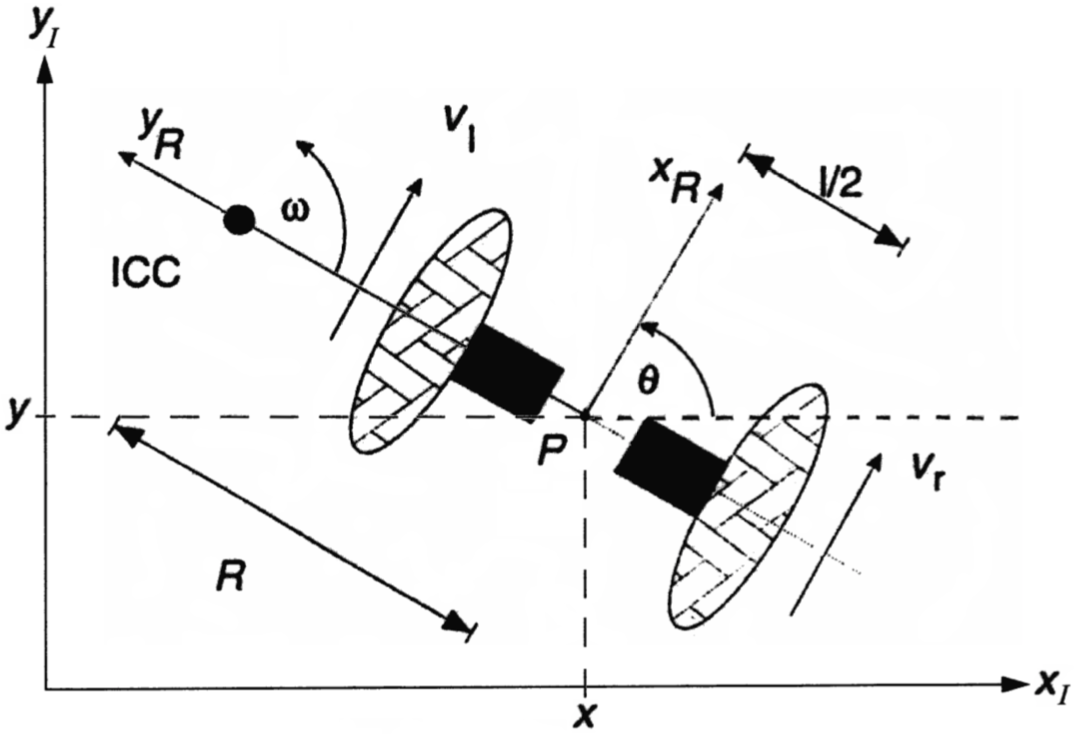
\includegraphics[width=0.7\textwidth]{figures/differential-drive-robot.png}\\
	\textbf{Synchro drive robot} has three steerable wheels that are parallel and turn with the same angle (to remain parallel) and rotate with the same velocity $\Rightarrow$ control inputs are velocity $v(t)$ and turning angle $\omega(t)$ (equations see lecture slides: chapter 07, slide 23ff)\\
	\textbf{Tricycle robot} has two fixed back wheels on the same axis and one steerable front wheel which is driven (there's is also a back wheel driven tricycle) $\Rightarrow$ control inputs are the steering angle $\alpha$ and the velocity $v$, fixed parameters are $l$ (distance between the back wheels) and $d$ (distance between the back axis and the front axis) (equations see lecture slides: chapter 07, slide 26ff)\\
	\textbf{Car-like robots/Ackermann steering} has two fixed back wheels that are driven on the same axis and two steerable front wheels. Since the steering angle of the two wheels relate to each other (to get an ICC) the model can be reduced to a back wheel driven tricycle which steering angle can be computed from one of the real steering angles $\Rightarrow$ control inputs are the steering angles $\alpha_l$ and $\alpha_r$ and the velocity $v$, fixed parameters are $l$ (distance between the back wheels) and $d$ (distance between the back axis and the front axis) (equations see lecture slides: chapter 07, slide 32ff)
	
	% TODO print lecture slides, chapter 07
	
	\subsection{Kinematic parameters}
	The kinematic parameters are used to specify the exact characteristics of a certain robot:
	\begin{itemize}
		\item $P$ is the reference point located on the robot
		\item $A$ mounting point of a wheel where it is connected to the robot case
		\item $l$ distance between $P$ and $A$
		\item $\alpha$ angle between $x_R$ and $\vec{PA}$
		\item $\beta$ angle between $\vec{PA}$ and the wheel axis
		\item $\varphi$ angular position of the wheel
		\item $r$ radius of the wheel
		\item $d$ offset between mounting and wheel center (only castor or off-centered steering wheel)
		\item $\gamma$ angle of rollers between wheel plane and rollers' axis (only Mecanum/Swedish)
	\end{itemize}
	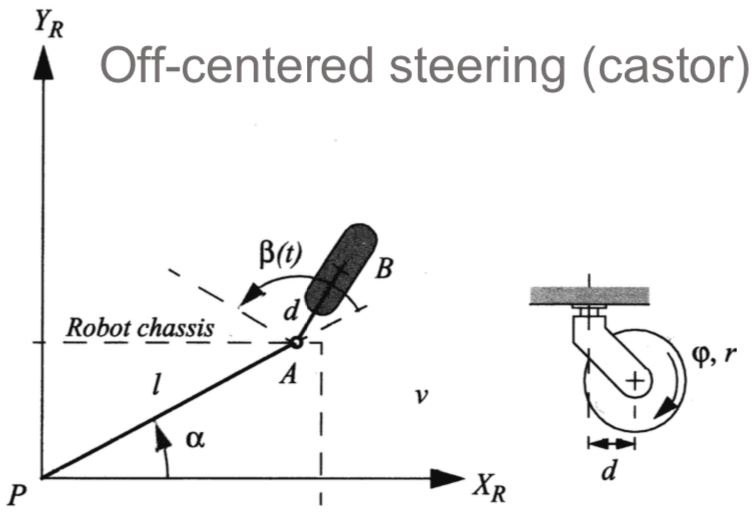
\includegraphics[width=0.5\textwidth]{figures/example-kinematic-parameters.png}
	
	\subsection{Direct kinematics}
	Direct kinematics is the determination of the robots coordinates and orientation in the base coordinate frame when the values for the velocities and the steering angles are given.\\
	\textbf{Coordinate frames} The inertial frame or base frame is called $L_I = {x_I, y_I}$ and the robot's frame is called $L_R = {x_R, y_R}$ (with $x_R$ aligned in the direction of movement)\\
	\textbf{Robot's pose} is described by a vector $p(t)$ with $x$, $y$ denoting the position of $P$ in $L_I$ and $\theta$ as the rotation angle of $L_R$ w.r.t. $L_I$.
	$$p(t) =
	\begin{bmatrix}
	x(t)\\
	y(t)\\
	\theta(t)
	\end{bmatrix}$$
	\textbf{Frame rotation} coordinates from $L_I$ can be converted to $L_R$ with $R(\theta)$ and with $R^{-1}(\theta)$ vice versa.
	$$R_R^I(\theta) = R(\theta) = 
	\begin{bmatrix}
	\cos \theta & \sin \theta & 0\\
	-\sin \theta & \cos \theta & 0\\
	0 & 0 & 1
	\end{bmatrix},
	R_I^R(\theta) = R^{-1}(\theta) = 
	\begin{bmatrix}
	\cos \theta & -\sin \theta & 0\\
	\sin \theta & \cos \theta & 0\\
	0 & 0 & 1
	\end{bmatrix}$$
	\textbf{Kinematic model} describes the "pose velocity" $\dot{p}(t)$ with the control inputs. To obtain the pose $p(t)$ integrate the kinematic model.\\
	Example for differential drive robot:
	$$\dot{p}(t) = \dot{p}_I(t) = R^{-1}(\theta) \dot{p}_R(t) = R^{-1}(\theta)
	\begin{bmatrix}
	v(t)\\
	0\\
	\omega(t)
	\end{bmatrix} = 
	\begin{bmatrix}
	v(t) \cos \theta(t)\\
	v(t) \sin \theta(t)\\
	\omega(t)
	\end{bmatrix}$$
	$$p(t) = 
	\begin{bmatrix}
	x(t)\\
	y(t)\\
	\theta(t)
	\end{bmatrix} = 
	\begin{bmatrix}
	x(0) + \int_{0}^{t} v(\tau) \cos \theta(\tau) d \tau\\
	y(0) + \int_{0}^{t} v(\tau) \sin \theta(\tau) d \tau\\\
	\theta(0) + \int_{0}^{t} \omega(\tau) d \tau
	\end{bmatrix}$$
	
	\subsection{Inverse kinematics}
	Inverse kinematics describes the task to determine the robot's control inputs (velocities, steering angles) when the desired pose (coordinates and orientation) is given. Not all poses can be reached with one set of control inputs. It has to be on a circle or straight line to the robot's original pose.\\
	To achieve the inputs to arbitrary poses, split the motion into segments where only some of the inputs are varied (e.g. rotation, straight line motion, rotation).\\
	Example for differential drive: Move from $[x_0, y_0, \theta_0]^T$ to $[x_3, y_3, \theta_3]^T$
	\begin{enumerate}
		\item $[x_0, y_0] = [x_1, y_1]$, $\tan \theta_1 = \frac{y_3 - y_0}{x_3 - x_0} \Rightarrow \theta_1 = \arctan2(y_3 - y_0, x_3 - x_0)$\\
		$v_r = -v_l = v_1 \Rightarrow \delta t_1 = \frac{(\theta_1 - \theta_0)l}{2 v_1}$
		\item $[x_2, y_2] = [x_3, y_3]$, $v_r = v_l = v_2 \Rightarrow \delta t_2 = \frac{\sqrt{(x_2 - x_0)^2 + (y_2 - y_0)^2}}{v_2}$
		\item $[x_2, y_2] = [x_3, y_3]$, $v_r = -v_l = v_3 \Rightarrow \delta t_3 = \frac{(\theta_3 - \theta_1)l}{2 v_3}$
	\end{enumerate}

	\subsection{Robot's constraints}
	\textbf{Holonomic constraints} do not depend on the velocity $\dot{q}$ but on the pose $p$. They reduce the number of generalized coordinates by one.\\
	\textbf{Holonomic robots} can control the total DOFs. (can be achieved with swedish or omnidirectional wheels)\\
	\textbf{Non-holonomic constraints} depend on the velocity $\dot{q}$ and the pose $p$.\\
	\textbf{Non-holonomic robots} can control less than the total numbers of DOFs. (this applies to all presented robots, because $\dot{y}_R = 0$)
	$$\begin{bmatrix}
	\dot{x}_R(t)\\
	\dot{y}_R(t)\\
	\dot{\theta}_R(t)\\
	\end{bmatrix} = 
	\begin{bmatrix}
	\cos \theta & \sin \theta & 0\\
	-\sin \theta & \cos \theta & 0\\
	0 & 0 & 1
	\end{bmatrix}
	\begin{bmatrix}
	\dot{x}(t)\\
	\dot{y}(t)\\
	\dot{\theta}(t)\\
	\end{bmatrix} = 
	\begin{bmatrix}
	\dot{x}(t) \cos \theta(t) + \dot{y}(t) \sin \theta(t)\\
	-\dot{x}(t) \sin \theta(t) + \dot{y}(t) \cos \theta(t)\\
	\dot{\theta}(t)\\
	\end{bmatrix}$$
	$$\Rightarrow G(q, \dot{q}, t) = -\dot{x}(t) \sin \theta(t) + \dot{y}(t) \cos \theta(t) = 0$$
	\textbf{Wheel constraint} a wheel should not slide in $y$ direction. This can be checked with:
	$$\dot{x}_R \cos(\alpha + \beta) + \dot{y}_R \sin(\alpha + \beta) + l \dot{\theta} \sin \beta = 0$$
	A wheel should also not slip in $x$ direction. This can be checked with:
	$$-\dot{x}_R \sin(\alpha + \beta) + \dot{y}_R \cos(\alpha + \beta) + l \dot{\theta} \cos \beta + r \dot{\varphi} = 0$$
	(for castor and Swedish wheels, see chapter 07, slide 57ff)\\
	\textbf{Kinematic constraints} To determine if the robot is sliding or slipping, all wheel constraints can be formalized in matrix form (see chapter 07, slide 61ff) which has then to be 0 to proof the existence of an ICC.\\
	To get the number of independent constraints, calculate: $rank(C_1^*(\beta_S))$\\
		
	\subsection{Classification}
	\textbf{Degree of mobility} measures the number of DOFs that can immediately be manipulated through changes of the wheel velocities: $\delta_m = 3 - rank(C_1^*(\beta_S))$ with $0 \leq \delta_m \leq 3$\\
	\textbf{Degree of steerability} measures the number of DOFs that can immediately be manipulated through changes of the steering angles. That equals to the number of independently controllable steering angles: $\delta_s = rank(C_{1s}(\beta_s))$\\
	\textbf{Degree of Maneuverability} is the sum of the DOFs that a robot can manipulate: $\delta_M = \delta_m + \delta_s$\\
	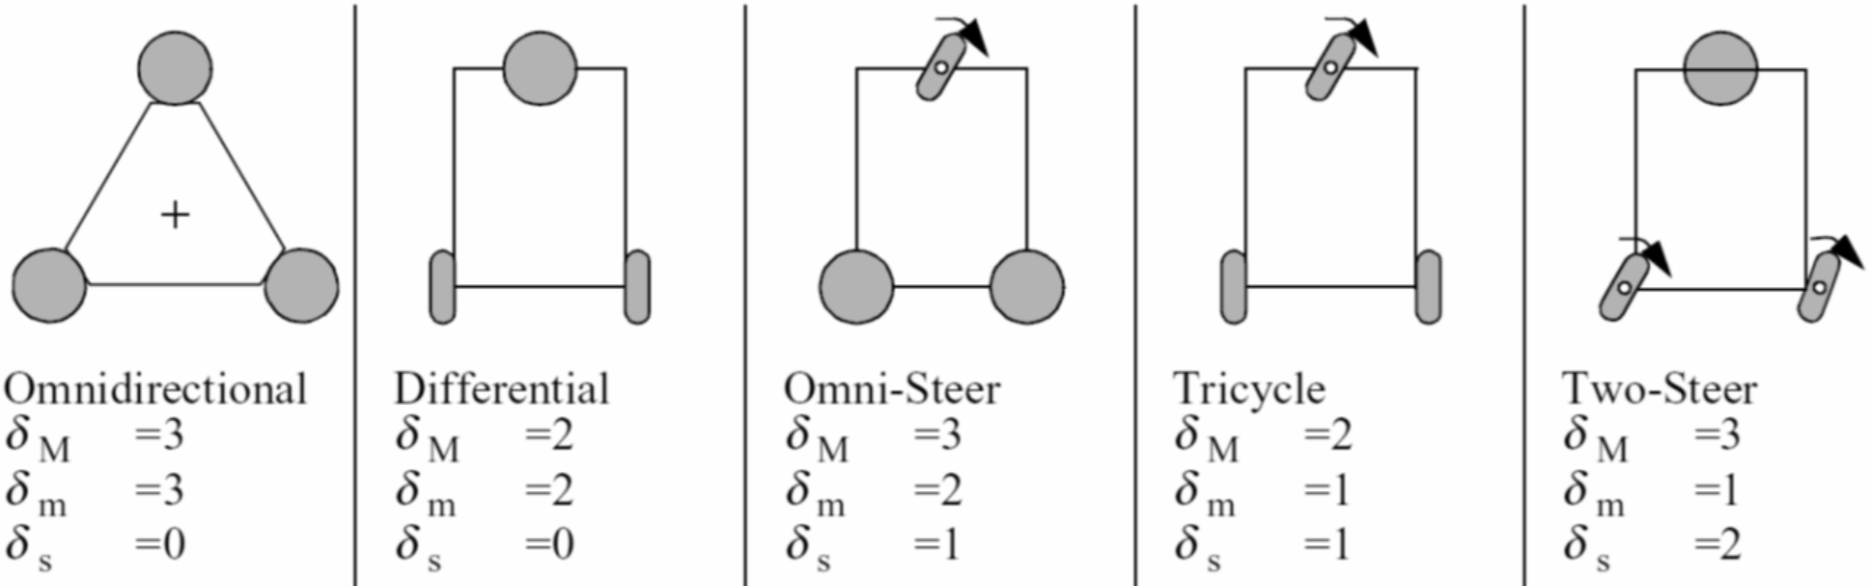
\includegraphics[width=\linewidth]{figures/robots-dofs.png}\\
	If $\delta_M = 2$ the ICC is constraint to a line, if $\delta_M = 3$ it can be chosen arbitrarily. If a robot has more than one fixed wheel they have to be on the same axis which can't be the axis of the steering wheels.\\
	\textbf{Classification} is done by the tuple of $(\delta_m, \delta_s)$\\
	\\
	\textbf{Follow the carrot} Method of reaching a goal that keeps the robot moving\\
	current position: $(x, y, \theta)^T$, goal position: $(x_L, y_L)^T$\\
	$\delta x = x_L - x$\\
	$\delta y = y_L - y$\\
	$\theta_L = \arctan2(\delta y, \delta x)$
	
	% TODO continue with chapter 08
\end{document}
